\chapter{Il percorso di stage }\label{cap:Il_percorso}
\section{Formazione}
Il processo di formazione ha avuto un ruolo fondamentale nella buona riuscita del progetto di stage, con una durata complessiva di circa quattro settimane. \\
La causa del protrarsi del processo di formazione è stata provocata dalla mia inesperienza in merito a 
concetti legati all'architettura \gls{eda}{},
\textbf{Apache Kafka}, \textbf{Apache Druid} e \textbf{Docker Compose}.\\  
Tutto il processo di formazione è stato tracciato e monitorato da me medesimo e dal tutor aziendale, attraverso le \gls{board}{} offerte 
dal software di \gls{project management}{} \textbf{ClickUp} (Figura \ref{cap:ClickUp}).\\
\begin{figure}[h]
    \centering
    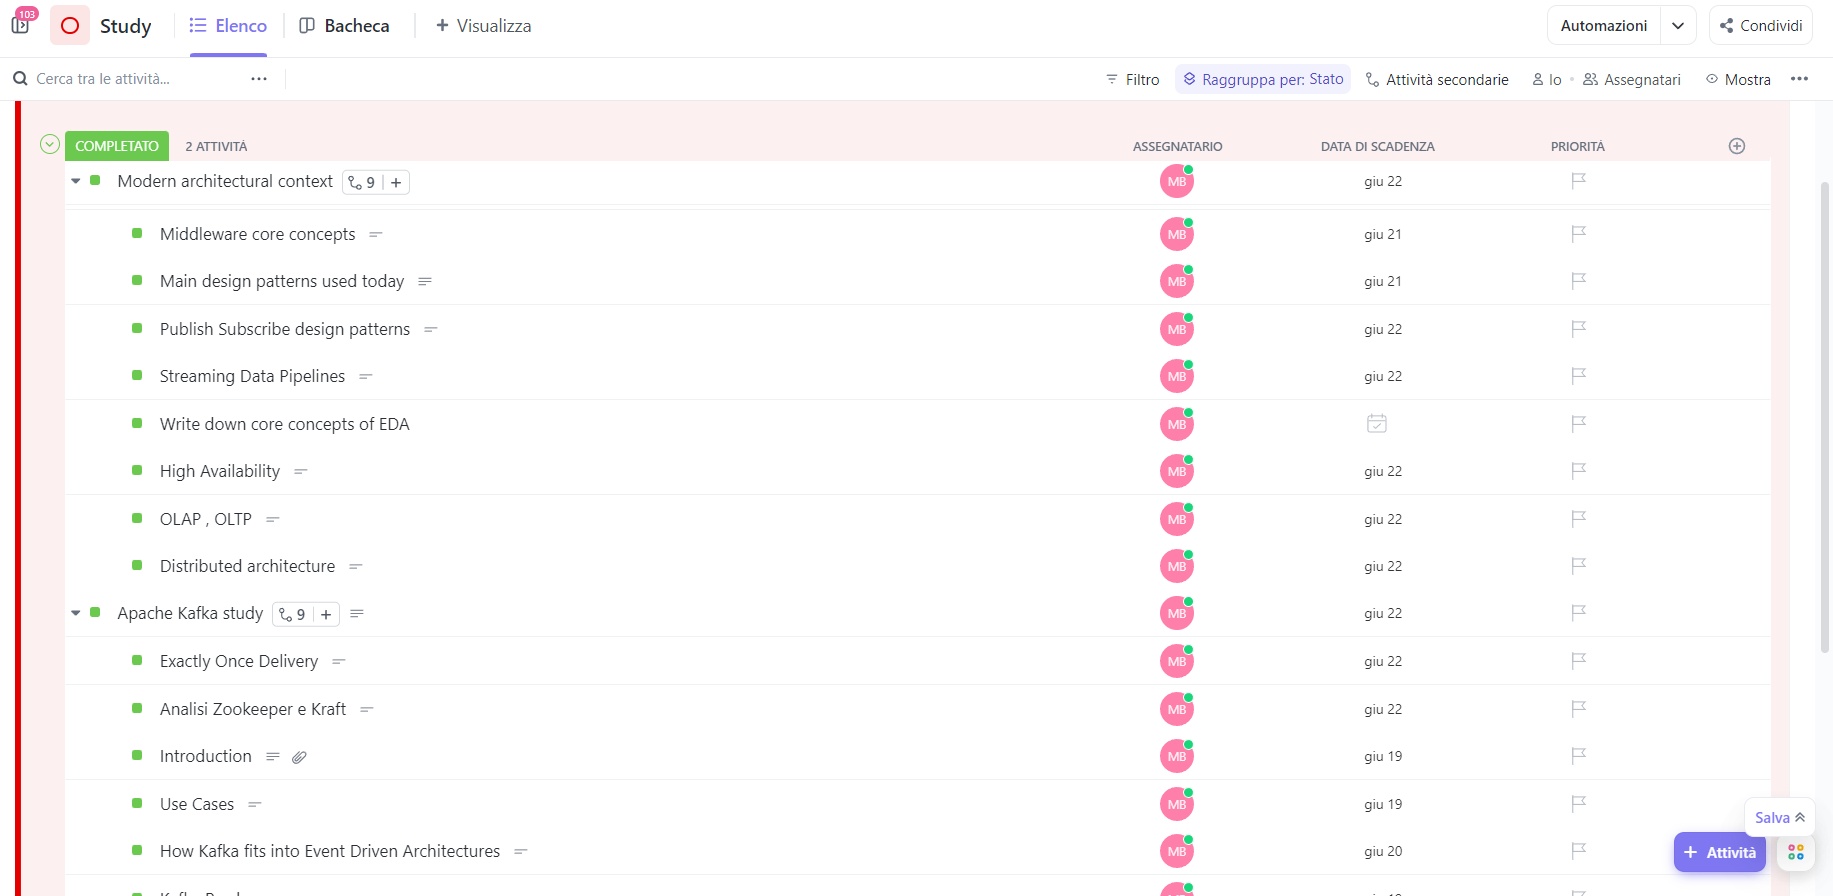
\includegraphics[width=1\textwidth]{images/percorso/formazione.png}
    \caption{Board di ClickUp per il processo di formazione}
    \label{cap:ClickUp}
\end{figure}
\pagebreak
\\
Inoltre durante il processo di formazione, oltre a reperire informazioni da documentazione ufficiale, ho avuto anche modo 
di approfondire quanto appena appreso attraverso delle attività di \gls{hands-on}{} che mi hanno permesso di mettere in pratica nell'immediato quanto appreso
(Figura \ref{cap:Hands-on}).
\begin{figure}[h]
    \centering
    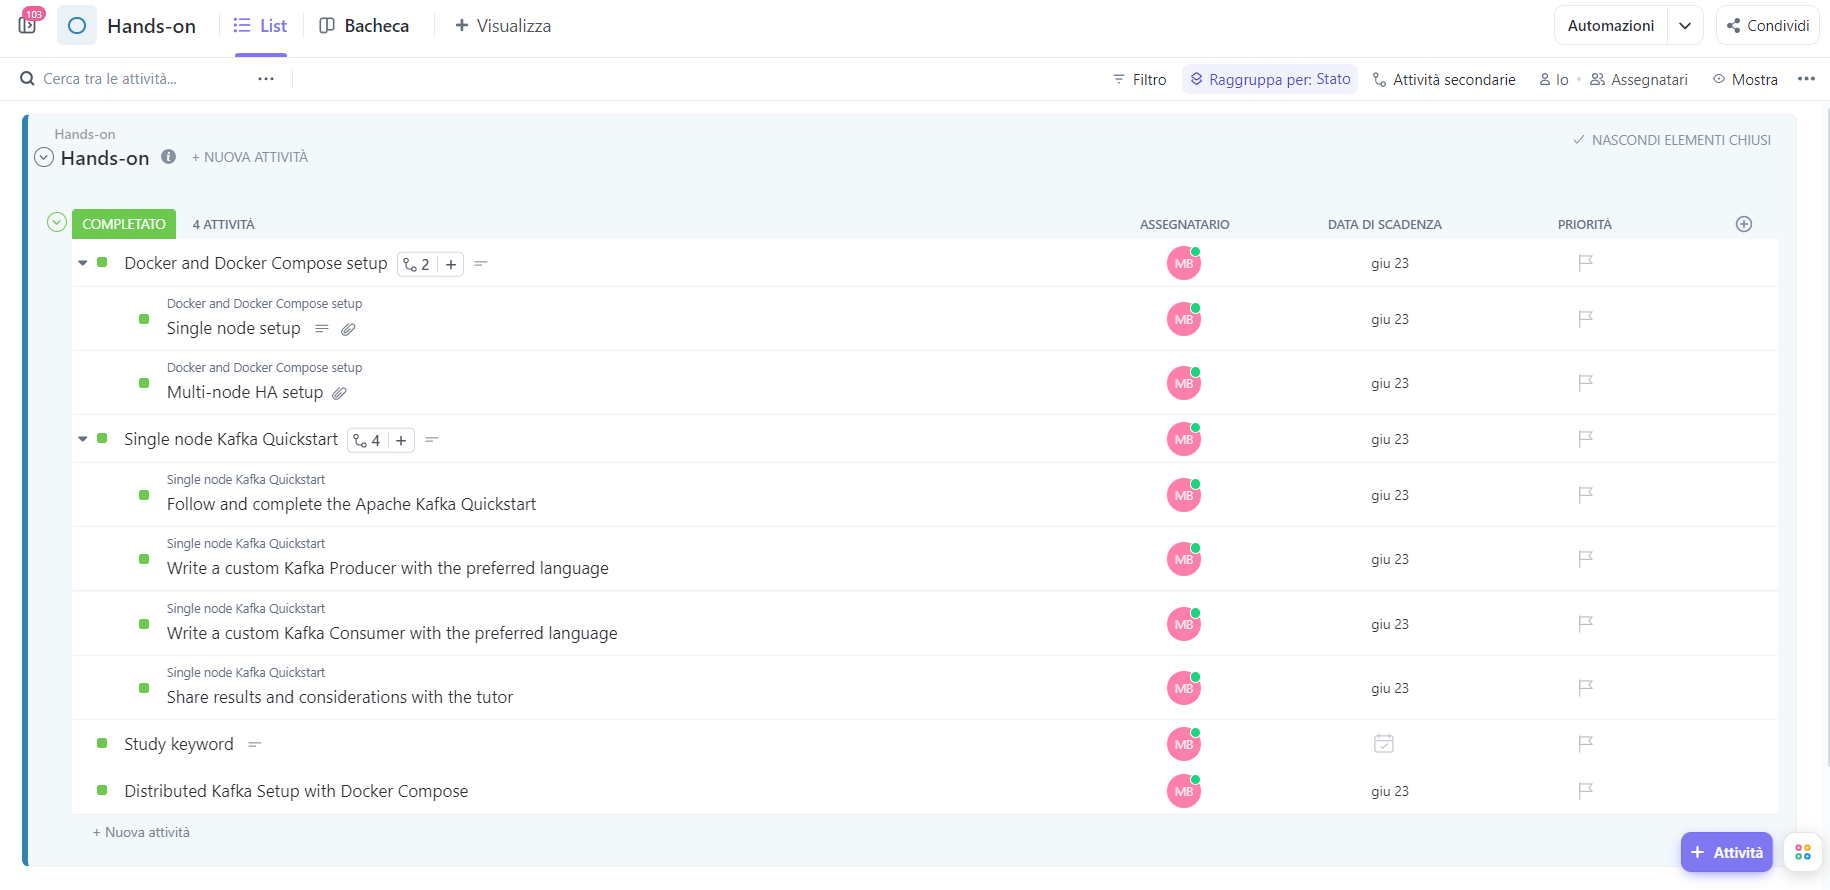
\includegraphics[width=1\textwidth]{images/percorso/hands_on.png}
    \caption{Attività di hands-on per il processo di formazione}
    \label{cap:Hands-on}
\end{figure}
\\
Durante il processo di formazione, in collaborazione con il tutor aziendale, è stato anche definito un processo di coordinamento e produzione di 
documentazione che mi ha permesso, durante tutto lo svolgimento del percorso di stage, di avere un tracciamento dei concetti appresi e 
 di avere un riferimento per un'eventuale risoluzione di problemi o dubbi sorti (Figura \ref{cap:Documentazione}).
\begin{figure}[h]
    \centering
    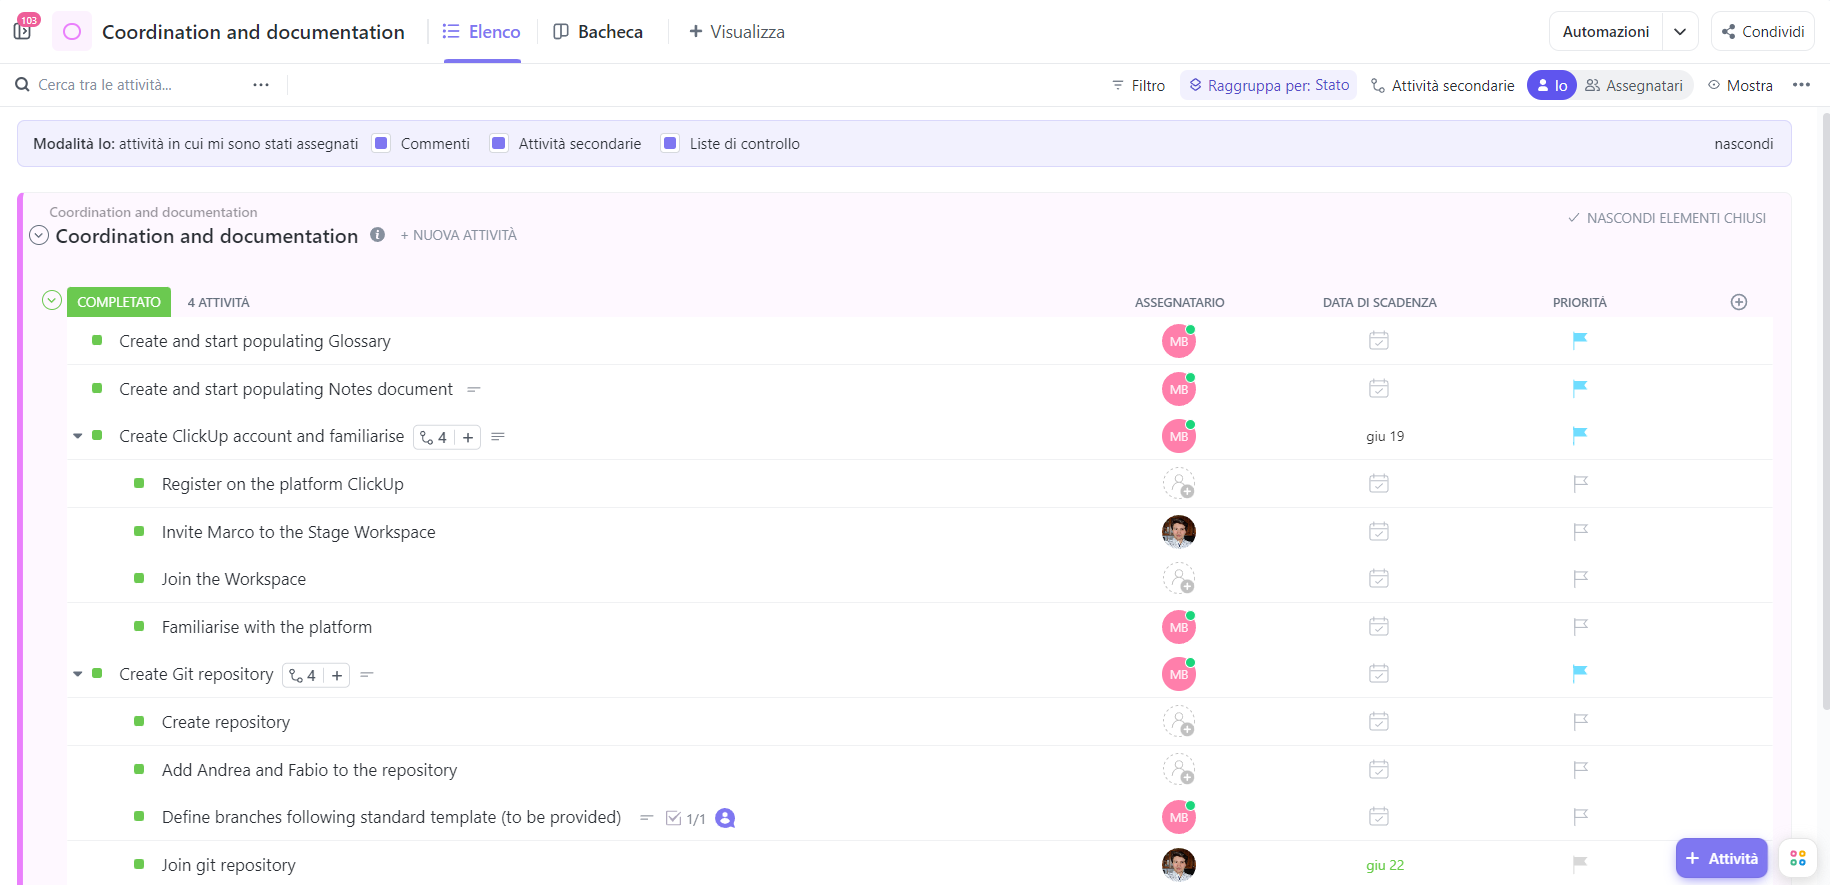
\includegraphics[width=1\textwidth]{images/percorso/coordinamento.png}
    \caption{Board di ClickUp per il processo di coordinamento e documentazione}
    \label{cap:Documentazione}
\end{figure}
\subsection{Daily stand-up meeting}
In ausilio dei processi sopra descritti, 
è stato anche definito, in concomitanza con l'inizio del processo di formazione, un processo di \textbf{supporto} ispirato al metodo \gls{Scrum}{}, 
andando a programmare degli incontri giornalieri di circa 15 minuti finalizzati a:
\begin{list}{*}
    \item \textbf{monitorare} lo stato di avanzamento delle attività svolte, da svolgere e in corso di svolgimento;
    \item \item \textbf{risolvere} eventuali dubbi o problemi sorti durante lo svolgimento delle attività;
    \item \textbf{definire} eventuali miglioramenti o cambiamenti da apportare alle attività da svolgere, o in corso di svolgimento, e al metodo 
    di lavoro adottato.
\end{list}
\section{Codifica}
\subsection{Configurazione di un cluster Kafka con Docker Compose}
Dopo aver terminato le attività di formazione su \textbf{Apache Kafka} e \textbf{Docker Compose} 
ho iniziato la configurazione di un \gls{cluster}{}, che fa uso di \gls{container}{}, in grado di testare tali strumenti.
\\Seguendo la buona pratica dell'alta affidabilità, descritta del 
paragrafo \ref{sec:alta_affidabilita}, ho configurato un \gls{cluster}{} con tre nodi \textbf{Kafka} e un nodo \textbf{Zookeeper}.\\
Innanzitutto per far che ogni \gls{container}{} possa comunicare con gli altri è stato necessario creare una 
\gls{Docker network}{}, denominata \textbf{kafka-druid}.
\begin{lstlisting}[caption=\texttt{docker network create}, label=1000st:file]{docker network create}
docker network create kafka-druid
\end{lstlisting}
Successivamente sono stati creati i nodi \textbf{Zookeeper} e \textbf{Kafka} con \textbf{Docker Compose} 
come illustrato nel listato \ref{90st:file} (per motivi di spazio viene riportata la definizione di un solo nodo \textbf{Kafka}, la configurazione degli altri è del tutto analoga).
\begin{lstlisting}[caption=\texttt{kafka-cluster-compose.yml}, label=90st:file]{kafka-cluster-compose.yml}
networks:
  kafka-druid:
    name: kafka-druid
    driver: bridge
    external: true
services:
  kafka:
    image: confluentinc/cp-kafka:7.4.0
    hostname: kafka
    container_name: kafka
    networks:
      - kafka-druid
    ports:
      - "29092:29092"
    environment:
      KAFKA_ADVERTISED_LISTENERS: INTERNAL://kafka:9092,EXTERNAL://localhost:29092
      KAFKA_LISTENER_SECURITY_PROTOCOL_MAP: INTERNAL:PLAINTEXT,EXTERNAL:PLAINTEXT
      KAFKA_INTER_BROKER_LISTENER_NAME: INTERNAL
      KAFKA_ZOOKEEPER_CONNECT: "zookeeper:2181"
      KAFKA_BROKER_ID: 1
      KAFKA_LOG4J_LOGGERS: "kafka.controller=INFO,kafka.producer.async.DefaultEventHandler=INFO,
      state.change.logger=INFO"
      KAFKA_OFFSETS_TOPIC_REPLICATION_FACTOR: 1
      KAFKA_TRANSACTION_STATE_LOG_REPLICATION_FACTOR: 1
      KAFKA_TRANSACTION_STATE_LOG_MIN_ISR: 1
      KAFKA_AUTHORIZER_CLASS_NAME: kafka.security.authorizer.AclAuthorizer
      KAFKA_ALLOW_EVERYONE_IF_NO_ACL_FOUND: "true"
\end{lstlisting}
È importante sottolineare che all'interno della configurazione, sopra descritta, 
vengono utilizzate le \gls{immagini Docker}{} \textbf{confluentinc/cp-zookeeper:7.4.0} e \\\textbf{confluentinc/cp-kafka:7.4.0}.\\
Tale scelta è stata adottata, dal fatto che oramai \textbf{Confluent} 
è diventata una distribuzione molto all' avanguardia, in quanto fornisce soluzioni, utilizzate anche a livello aziendale,
per la gestione di flussi di dati in tempo reale, come in Sync Lab.\\
Nonostante ciò si precisa che per i test che verranno elencati di seguito,
sono utilizzabili anche le \gls{immagini Docker}{} ufficiali di \textbf{Apache Kafka} e \textbf{Apache Zookeeper}, distribuite dalla 
\gls{Apache Software Foundation}.
\subsection{Configurazione del file di enviroment per il cluster di Apache Druid}
Dopo aver configurato il \gls{cluster}{} di \textbf{Apache Kafka}, è stato necessario adattarne il file di \gls{enviroment}{} di \textbf{Apache Druid}, come descritto nel listato \ref{8st:file}.
\begin{lstlisting}[caption=\texttt{enviroment}, label=8st:file]{enviroment}
DRUID_MAXDIRECTMEMORYSIZE=3072m
DRUID_SINGLE_NODE_CONF=nano-quickstart
druid_emitter_logging_logLevel=debug
druid_extensions_loadList=["druid-histogram", "druid-datasketches", "druid-lookups-cached-global", "postgresql-metadata-storage", "druid-multi-stage-query", "druid-kafka-indexing-service"]
druid_zk_service_host=zookeeper
druid_lookup_enableLookupSyncOnStartup=true
druid_lookup_lookupTierIsDatasource=false
druid_lookup_lookupTier=_default_tier
druid_broker_cache_useCache=true
druid_broker_cache_populateCache=true
druid_broker_cache_useResultLevelCache=true
druid_broker_cache_populateResultLevelCache=true
druid_cache_useCache=true
druid_cache_populateCache=true
druid_cache_useResultLevelCache=true
druid_cache_populateResultLevelCache=true
druid_metadata_storage_host=
druid_metadata_storage_type=postgresql
druid_metadata_storage_connector_connectURI=jdbc:postgresql://postgres:5432/druid
druid_metadata_storage_connector_user=druid
druid_metadata_storage_connector_password=FoolishPassword
druid_coordinator_balancer_strategy=cachingCost
druid_indexer_runner_javaOptsArray=["-server", "-Xmx1g", "-Xms1g", "-XX:MaxDirectMemorySize=3g", "-Duser.timezone=UTC", "-Dfile.encoding=UTF-8", "-Djava.util.logging.manager=org.apache.logging.log4j.jul.LogManager"]
druid_indexer_fork_property_druid_processing_buffer_sizeBytes=256MiB
druid_storage_type=local
druid_storage_storageDirectory=/opt/shared/segments
druid_indexer_logs_type=file
druid_indexer_logs_directory=/opt/shared/indexing-logs
druid_processing_numThreads=1
druid_processing_numMergeBuffers=1
DRUID_LOG4J=<?xml version="1.0" encoding="UTF-8" ?><Configuration status="WARN"><Appenders><Console name="Console" target="SYSTEM_OUT"><PatternLayout pattern="%d{ISO8601} %p [%t] %c - %m%n"/></Console></Appenders><Loggers><Root level="info"><AppenderRef ref="Console"/></Root><Logger name="org.apache.druid.jetty.RequestLog" additivity="false" level="DEBUG"><AppenderRef ref="Console"/></Logger></Loggers></Configuration>
\end{lstlisting}
Tale azione è stata resa necessaria dal fatto che \textbf{Apache Druid} è uno strumento \gls{olap}{}, che necessita di grandi quantità di memoria RAM e spazio su disco per operare 
su moli considerevoli di dati.\\
Pertanto si sottolinea, che nella configurazione sopra citata, viene utilizzata una versione di \textbf{Druid}, denominata \textbf{nano-quickstart}, che permette di utilizzare tale strumento con un consumo di risorse ridotto.
\subsection{Configurazione di un cluster di Apache Druid con Docker Compose}
Per la definizione del \gls{cluster}{} di \textbf{Apache Druid},
al fine di ottimizzare il consumo di memoria RAM necessaria per la sua esecuzione,
sono stati utilizzati un nodo per ogni processo di \textbf{Apache Druid}.
Nel file di configurazione, illustrato nel listato \ref{9st:file}, vengono definiti:
\begin{list}{*}
  \item  un nodo \textbf{Coordinator};
  \item \item  un nodo \textbf{Historical};
  \item  un nodo \textbf{Broker}; 
  \item  un nodo \textbf{MiddleManager}, implementato per mezzo di \textbf{PostgreSQL}.
\end{list} 
\pagebreak
\begin{lstlisting}[caption=\texttt{druid-cluster-compose.yml}, label=9st:file]{druid-cluster-compose.yml}
volumes:
  coordinator_var: {}
  druid_shared: {}
services:
  coordinator:
    image: apache/druid:26.0.0
    container_name: coordinator
    networks:
      - kafka-druid
    volumes:
      - druid_shared:/opt/shared
      - coordinator_var:/opt/druid/var
    depends_on:
      - zookeeper
      - postgres
    ports:
      - "8081:8081"
    command:
      - coordinator
    env_file:
      - environment
\end{lstlisting}
È importante sottolineare che all'interno del file di configurazione, sopra descritto, vengono definite anche 
i \gls{volumi}{} necessari per l'archiviazione dei dati e dei \gls{log}{}, essenziali al funzionamento del \gls{cluster}{}.
\subsection{Creazione del produttore di eventi Kafka}
Al fine di poter testare i \gls{cluster}{} appena creati, descritti nelle sezioni precedenti, ho creato 
un produttore di eventi \textbf{Kafka}, 
in grado d'instaurare una connessione con il \gls{cluster}{} di \textbf{Apache Kafka}, di 
generare eventi in modo casuale, secondo un determinato \textbf{schema} predefinito e d'inviarli al \gls{cluster}{}, sopra citato.
\\Per la creazione del produttore di eventi, è stato utilizzato il linguaggio di programmazione \textbf{Python}, la libreria \gls{Kafka-Python}{} e in particolare il modulo \textbf{KafkaProducer}, come illustrato nel listato \ref{l0st:file}.
\begin{lstlisting}[language=Python, caption=\texttt{producer.py}, label=l0st:file]{producer.py}
producer = KafkaProducer(  
  bootstrap_servers = ['localhost:29092'],  
  value_serializer = lambda x:json.dumps(x).encode('utf-8')  
  )  
\end{lstlisting}
È importante sottolineare che il produttore \textbf{Kafka} è stato creato in modo tale da inviare  eventi, associati al relativo \gls{topic}{} di appartenenza, in formato \gls{json}{},
alla porta pubblica, unica porta che può essere raggiunta dall'esterno
del \gls{message broker}{}, precedentemente configurato.
\pagebreak
\section{Esecuzione e testing}
Una volta configurato i \gls{cluster}{} sopra descritti, e aver creato una \gls{Data Pipeline}{}, come illustrato nella sezione \ref{sec:approccio_utilizzato}, 
per comprendere gli strumenti sopra citati, sono state eseguite delle attività di \textbf{testing}, finalizzate a:
\begin{list}{*}
    \item \textbf{verificare} le prestazioni di esecuzione di \textbf{Apache Druid}, all'interno di un \gls{cluster}{} \gls{Docker}{};
   \item  \item \textbf{evidenziare} le funzionalità che tale strumento può offrire.
\end{list}
\noindent
Per l'esecuzione dei \gls{cluster}{} è stato utilizzato l'apposito comando di \textbf{Docker Compose} (per motivi di spazio viene riportato solo 
l'esecuzione del \gls{cluster}{} di \textbf{Apache Druid}, Figura \ref{fig:druid_compose}).
\begin{figure}[h]
  \centering
  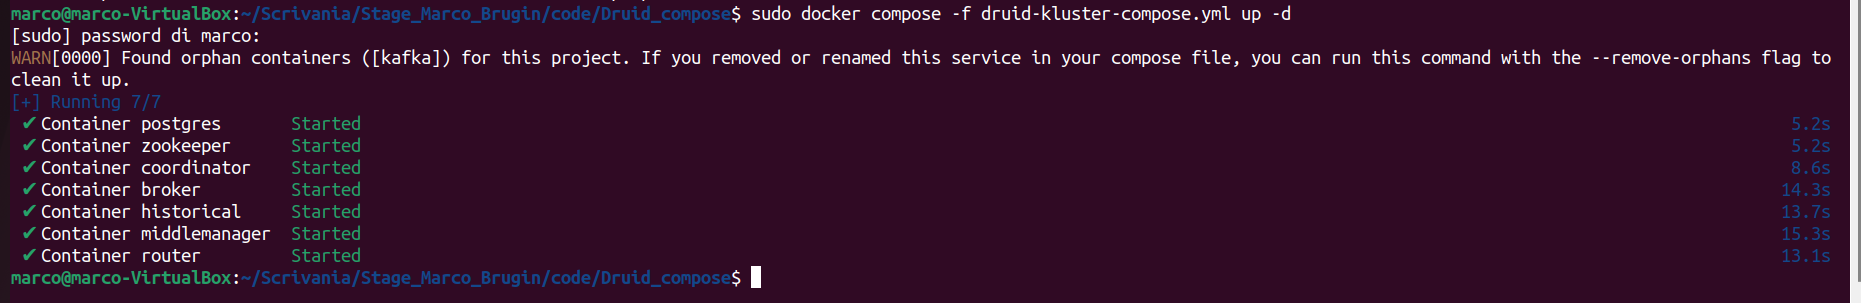
\includegraphics[width=1\textwidth]{images/percorso/druid_cluster.png}
  \caption{Esecuzione del cluster di Apache Druid con Docker Compose}
  \label{fig:druid_compose}
\end{figure}
\subsection{Creazione di una Data Pipeline}
\subsubsection{Confronto delle prestazioni di esecuzione tra Apache Druid e PostgreSQL}\label{sec:confronto_prestazioni1}
Al fine di mettere in risalto le prestazioni di \textbf{Apache Druid} e confrontarle con quelle ottenute da un classico database relazione, come \textbf{PostgreSQL}, è stato creato un \gls{datasource}{} di cinque milioni di record, a partire 
dal seguente schema relazionale.
\begin{lstlisting}[language=SQL]
  CREATE TABLE accessi( nome text, cognome text, indirizzo text, citta text, stato text, cap int, 
  email text, telefono text, eta int, altezza decimal(5,2), peso decimal(5,2), reddito decimal(6,2), 
  datan date, professione text, istruzione text, hobby text, nfigli int, codice_cliente int, datareg timestamp,__time timestamp)    
\end{lstlisting}
Si fa notare che all'interno del \gls{datasource}{} è presente un \textbf{timestamp} primario, denominato \textbf{\_\_time}, che viene utilizzato da \textbf{Apache Druid} per l'esecuzione 
efficiente delle query e il partizionamento dei dati all'interno dei segmenti di archiviazione.
\subsubsection{Svolgimento}
Per poter generare i dati necessari al \gls{datasource}{} è stato utilizzato il produttore di eventi, sopra descritto e la libreria \gls{Faker}{}, utilizzando i seguenti metodi (per motivi di spazio viene riportata nel listato \ref{30st:file} solo la generazione 
dei campi nome e cognome del \gls{datasource}{}).
\pagebreak
\begin{lstlisting}[language=Python, caption=\texttt{producer.py}, label=30st:file]{producer.py}
fake = Faker()
max=random.randint(4,20)  
nomi= [fake.first_name() for _ in range(max)]
max=random.randint(4,20)
cognomi= [fake.last_name() for _ in range(max)]
for n in range(500):
    for j in range(10000):
      nome= random.choice(nomi)
      cognome= random.choice(cognomi)
      my_data = {"nome": nome, "Cognome": cognome
      }
      producer.send("accessi", value = my_data) 
\end{lstlisting}
Inoltre per far si che il test eseguito sia il più veritiero possibile, tutti i dati generati 
sono stati salvati in un file denominato \textbf{data.csv} e successivamente importati all'interno di \textbf{PostgreSQL}, come illustrato nel listato \ref{20st:file}.
\begin{lstlisting}[language=SQL, caption=\texttt{import\_psql.sql}, label=20st:file]{import_psql.sql}
  COPY accessi(nome, cognome, indirizzo, citta, stato, cap, email, telefono, eta, altezza, peso, reddito, datan, professione, istruzione, hobby, nfigli, codice_cliente, datareg, __time)
  From '/data.csv'
  Delimiter ','
  csv header;
\end{lstlisting}
Si fa notare che i comandi, citati nel listato \ref{20st:file}, sono stati eseguiti solo dopo
aver aperto una connessione all'unico database, presente nel \gls{container}{} \textbf{postgres}, denominato \textbf{druid}, avente come password e nome utente \textbf{druid} (Figura \ref{fig:accesso_psql}).
\begin{figure}[h]
  \centering
  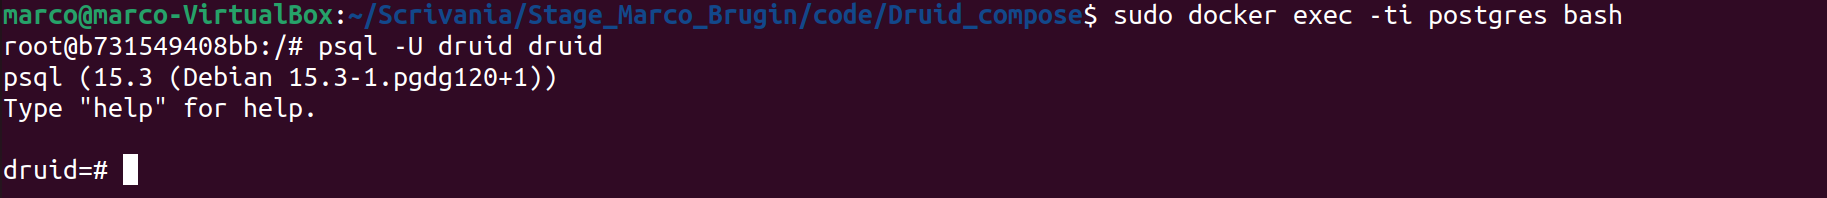
\includegraphics[width=1\textwidth]{images/percorso/accesso_psql.png}
  \caption{Connessione al database druid all'interno del container postgres}
  \label{fig:accesso_psql}
\end{figure}
\\
In seguito è stato anche eseguita l'\gls{injection}{} all'interno di \textbf{Apache Druid} 
andando a utilizzare l'interfaccia web, reperibile all'indirizzo
\textbf{http://localhost:8888/} (Figura \ref{fig:injection}).
\begin{figure}[h]
  \centering
  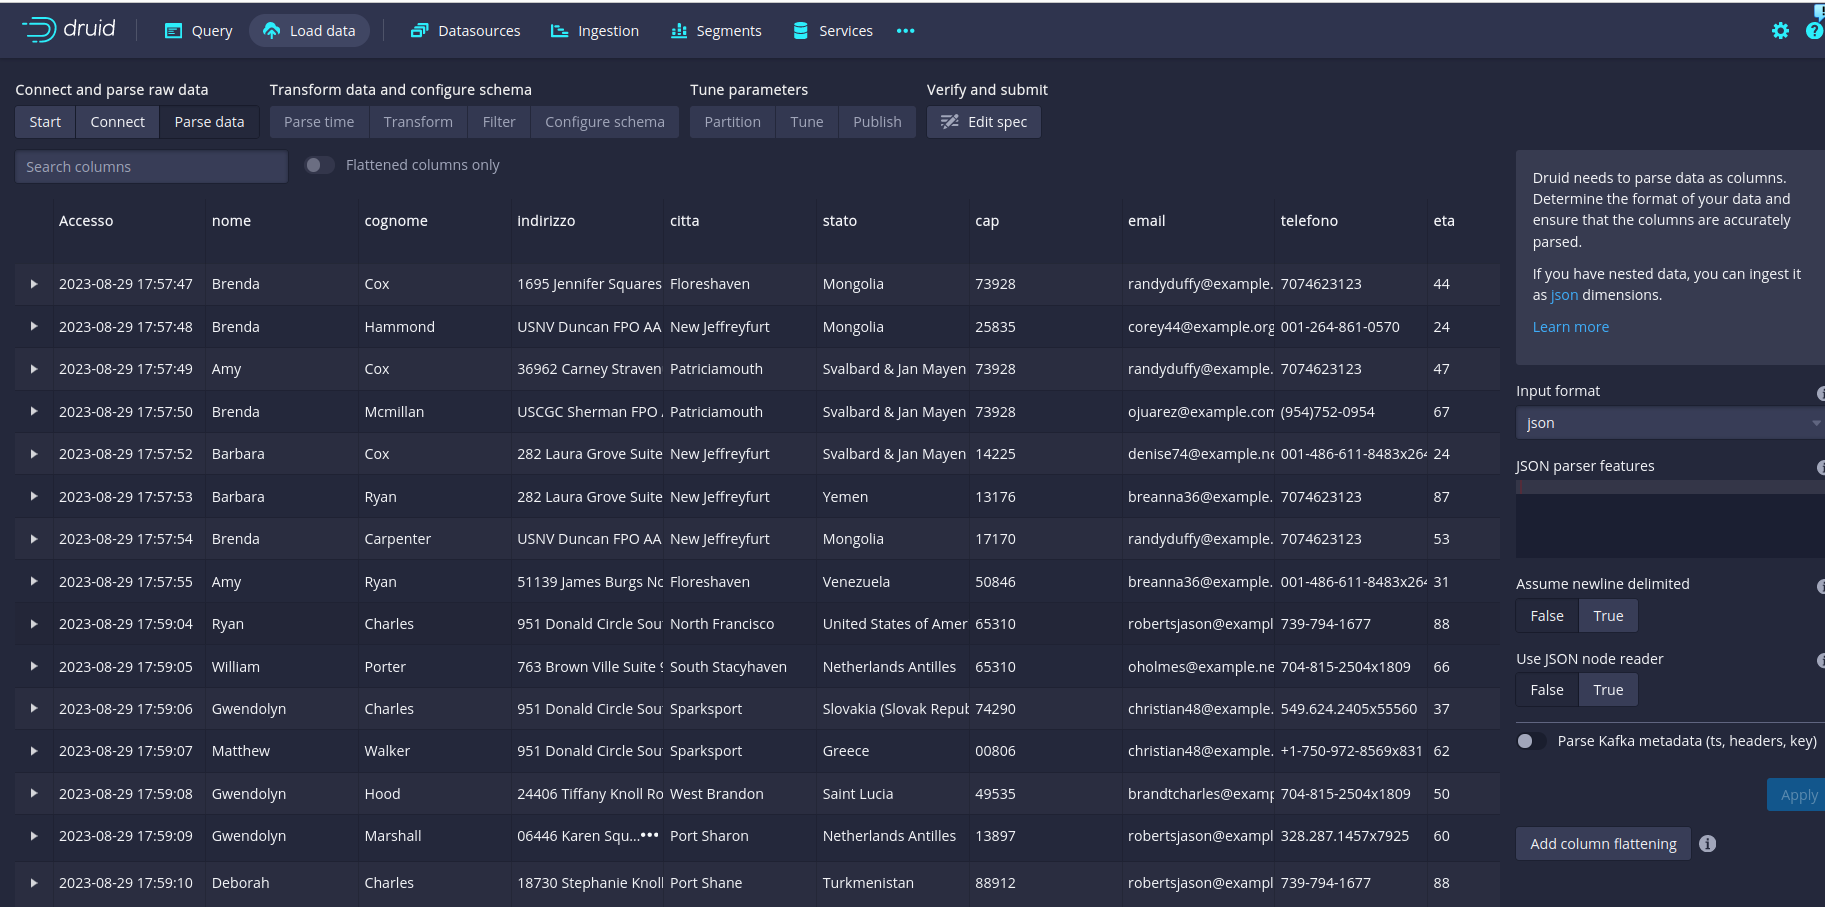
\includegraphics[width=1\textwidth]{images/percorso/load_data.png}
  \caption{Interfaccia web di Apache Druid per l'injection di un datasource}
  \label{fig:injection}
\end{figure}
\pagebreak
\\
Infine sono state eseguite le seguenti query \ref{89000st:file}, sia su \textbf{Apache Druid} che su \textbf{PostgreSQL}.
\begin{lstlisting}[language=SQL, caption=\texttt{query.sql}, label=89000st:file]{query.sql}
  - query 1:  SELECT DATE_TRUNC('day', __time), citta, COUNT(*)
              FROM accessi
              GROUP BY DATE_TRUNC('day', __time), citta
       
 - query 2:  SELECT stato, AVG(eta), AVG(reddito)
             FROM accessi
             GROUP BY stato
       
 - query 3:  SELECT DATE_TRUNC('year', __time), stato, professione, istruzione, nfigli, COUNT(*)
             FROM accessi
             WHERE nfigli> 0
             GROUP BY DATE_TRUNC('year', __time), stato, professione, istruzione, nfigli
             ORDER BY 5 DESC
       
 - query 4:  SELECT DATE_TRUNC('hour',__time), citta,  AVG(eta)
             FROM accessi
             GROUP BY DATE_TRUNC('hour', __time), citta  
 
 - query 5: SELECT DATE_TRUNC('year', __time), DATE_TRUNC('month', __time), DATE_TRUNC('day', __time),    stato, professione, istruzione, nfigli, COUNT(*) 
            FROM accessi
            GROUP BY DATE_TRUNC('year', __time), DATE_TRUNC('month', __time), DATE_TRUNC('day', __time), stato, professione, istruzione, nfigli
            ORDER BY 5 DESC



 - query 6:  SELECT DATE_TRUNC('year', __time), DATE_TRUNC('month', __time), DATE_TRUNC('day', __time), DATE_TRUNC('hour', __time), stato, professione, istruzione, nfigli, COUNT(*) 
             FROM accessi
             GROUP BY DATE_TRUNC('year', __time), DATE_TRUNC('month', __time), DATE_TRUNC('day', __time), DATE_TRUNC('hour', __time), stato, professione, istruzione, nfigli
             ORDER BY 5 DESC           
 \end{lstlisting}

\subsubsection{Risultati}
I risultati ottenuti sono riportati nella tabella \ref{tab:risultati_query}.
\begin{table}[h]
  \centering
  \caption{Risultati delle query eseguite su Apache Druid e PostgreSQL}
  \label{tab:risultati_query}
  \begin{tabular}{|c|c|c|}


\hline
& \textbf{Apache Druid [s]} &  \textbf{PostgreSQL [s]} \\\hline 

\textbf{query1} &    0.6 &  1.2 \\ \hline

\textbf{query2} &   0.2 &   1.9 \\ \hline 

\textbf{query3} &  1.2 &  2 \\ \hline
\textbf{query4} &  0.6 &  1.1 \\ \hline
\textbf{query5} &   1.05 &  2.8 \\ \hline
\textbf{query6} & 1.30 &  3.3 \\ \hline    
  \end{tabular}
\end{table}
\subsubsection{Considerazioni}
Dai risultati ottenuti si può notare che \textbf{Apache Druid} ha prestazioni migliori rispetto a \textbf{PostgreSQL}.\\
Tale risultato è dovuto al fatto che \textbf{Druid} nella esecuzione delle query va a utilizzare solo le colonne richieste, grazie al fatto che 
il \gls{datasource}{} viene archiviato per singole colonne.\\
Inoltre si può notare anche che il divario delle prestazioni tra i due strumenti aumenta nel momento 
in cui si eseguono query che coinvolgono operazioni sui timestamp primari.
Infatti in \textbf{Druid} i dati vengono archiviati secondo un partizionamento temporale definito 
al momento dell'\gls{injection}{}, che permette di eseguire le query in modo efficiente (vedi \ref{sec:deep_storage}).
\pagebreak
\subsubsection{Confronto delle prestazioni di esecuzione tra datasource con e senza rollup in Apache Druid}\label{sec:confronto_prestazioni2}
Con il termine di \textbf{Data rollup} si intende un'operazione di aggregazione eseguita 
sui dati, che permette di ridurre la dimensione di questi ultimi, andando a creare dei record di archiviazione più piccoli e migliorando così 
le prestazioni di esecuzione delle query.\\
In \textbf{Apache Druid} l'operazione di \textbf{rollup}, viene eseguita attraverso la 
definizione di segmenti aggregati, creati in base a delle regole di aggregazione configurate al momento dell'\gls{injection}{} del \gls{datasource}{}, direttamente dall'interfaccia web di \textbf{Apache Druid} (Figura \ref{fig:rollup}).
\begin{figure}[h]
  \centering
  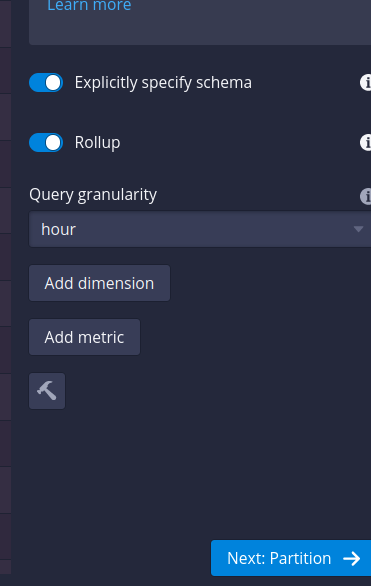
\includegraphics[width=0.3\textwidth]{images/percorso/test_rollup.png}
  \caption{Attivazione funzionalità di rollup all'interno di Apache Druid}
  \label{fig:rollup}
\end{figure}
\\
È importante sottolineare che l'operazione di \textbf{rollup} può essere configurata in base 
alla granularità temporale desiderata: si possono aggregare record aventi la stessa ora, minuti o secondi e considerando in seguito i  valori degli altri campi.\\
In generale \textbf{Apache Druid} offre, a seconda del metodo d' importazione dei dati, due metodi differenti di \textbf{rollup}:
\begin{list}{*}
  \item \textbf{rollup  perfetto}: \textbf{Apache Druid} aggrega perfettamente i dati al momento dell'\gls{injection}{};
  \item \item \textbf{best-effort rollup}: \textbf{Druid} potrebbe non riuscire ad aggregare perfettamente i dati 
  di input, pertanto si potrebbe verificare che più segmenti dati contengano dati con
  stesso \textbf{timestamp} e stesso valore di \textbf{Dimension}.
\end{list}
\noindent
Al fine di garantire il \textbf{rollup perfetto}, ottenendo così le prestazioni migliori, è necessario utilizzare un metodo d'inserimento 
che utilizzi un ulteriore passaggio di pre-elaborazione dei dati, finalizzato a determinare gli intervalli e il partizionamento da adottare 
al momento dell'inserimento dei dati. \\
Tale fase esegue una scansione dell'intero set d'input e aumenta il tempo necessario per l'inserimento.
\\Mentre una caratteristica tipica di un metodo d'inserimento che utilizza il \textbf{best-effort rollup} è la pubblicazione incrementale dei dati.
In questo \textbf{Apache Druid} finalizza e pubblica i segmenti prima che tutti i dati di una partizione temporale siano stati ricevuti. 
 \pagebreak   \\Tutte le importazioni dati, provenienti da \textbf{Streaming} avvengono in questo modalità.\\
\noindent Per mettere in risalto la funzionalità appena descritta ho creato un \gls{datasource}{} di cinque milioni di record, come illustrato nel listato \ref{11st:file}.
\begin{lstlisting}[language=SQL, caption=\texttt{table\_rollup.sql},label=11st:file]
    CREATE TABLE accessi_rollup(__time timestamp, nome text, cognome text, citta text, stato text, datan date, istruzione text, hobby text)
\end{lstlisting}
In questo caso si tratta di un modello molto semplice 
e per riuscire ad apprezzare la funzionalità di \textbf{rollup} è stato ridotto
il numero di possibili valori, che ogni campo dati può assumere.\\
Pertanto il confronto è stato eseguito tra il \gls{datasource}{} originale e quello a cui è stata applicata la funzionalità di \textbf{rollup}.\\
Inoltre, per completezza, tutti i dati generati sono stati salvati e importati anche all'interno di \textbf{PostgreSQL} per avere 
anche un confronto con un classico \textbf{database relazionale}.
 
\pagebreak
\subsubsection{Svolgimento}
Per poter generare i dati necessari al \gls{datasource}{} sopra descritto, 
è stato utilizzato il produttore di eventi e la libreria \gls{Faker}{}, come illustrato nel listato \ref{l9st:file}.
\begin{lstlisting}[language=Python, caption=\texttt{producer\_rollup.py}, label=l9st:file]{producer.py}
  fake = Faker()
  locazione=[[fake.city(), fake.country()] for _ in range(200)]
  utenti=list()
  num_utenti=5000
  for i in range(num_utenti):
      loc=locazione[random.randint(0,199)]
      citta=loc[0]
      stato=loc[1]
      utenti.append([fake.first_name(), fake.last_name(),fake.date_of_birth(minimum_age=18, maximum_age=89).strftime("%Y-%m-%d"), citta, stato, fake.random_element(elements=("Scuola Secondaria", "Laurea triennale", "Laurea Magistrale", "Dottorato")), fake.random_element(elements=("Leggere","Viaggiare","Giocare a calcio","Giocare ai videogiochi","Fare sport")) ] )
  for n in range(50):
    for j in range(100000):
        accesso=datetime.datetime.now().strftime("%Y-%m-%d %H:%M:%S")
        a=random.randint(0,4999)
        nome=utenti[a][0]
        cognome=utenti[a][1]
        datan=utenti[a][2]
        citta=utenti[a][3]
        stato=utenti[a][4]
        istruzione=utenti[a][5]
        hobby=utenti[a][6]
        my_data = {"__time": accesso, "nome": nome, "cognome": cognome, "datan":  datan, "citta": citta, "stato": stato, "istruzione": istruzione,
        "hobby": hobby
        }
        producer.send("accessi_rollup", value = my_data) 
    \end{lstlisting}
In seguito sono state eseguente le seguenti query \ref{800st:file} su i tre \gls{datasource}{} creati.
\begin{lstlisting}[language=SQL, caption=\texttt{query\_rollup.sql}, label=800st:file]{query_rollup.sql}
  - query 1: SELECT DATE_TRUNC('day', __time), citta, COUNT(*)
              FROM accessi_rollup
              GROUP BY DATE_TRUNC('day', __time), citta
              
  - query 2: SELECT DATE_TRUNC('year', __time), DATE_TRUNC('month', __time), stato, COUNT(*)
              FROM accessi_rollup
              GROUP BY DATE_TRUNC('year', __time), DATE_TRUNC('month', __time), stato
              ORDER BY 4 DESC
  


  - query 3: SELECT DATE_TRUNC('year', __time), DATE_TRUNC('month', __time), DATE_TRUNC('day', __time), stato, citta, COUNT(*) 
              FROM accessi_rollup
              GROUP BY DATE_TRUNC('year', __time), DATE_TRUNC('month', __time), DATE_TRUNC('day', __time), stato, citta
              ORDER BY 5 DESC
  
  - query 4: SELECT DATE_TRUNC('year', __time), DATE_TRUNC('month', __time), DATE_TRUNC('day', __time), DATE_TRUNC('hour', __time), stato, citta, COUNT(*) 
              FROM accessi_rollup
              GROUP BY DATE_TRUNC('year', __time), DATE_TRUNC('month', __time), DATE_TRUNC('day', __time), DATE_TRUNC('hour', __time), stato, citta
              ORDER BY 5 DESC
  \end{lstlisting}
\subsubsection{Risultati}
I risultati ottenuti sono riportati nella tabella \ref{tab:risultati_rollup}.
\begin{table}[h]
  \centering
  \caption{Risultati delle query eseguite con, senza rollup e su PostgreSQL}
  \label{tab:risultati_rollup}
  \begin{tabular}{|c|c|c|c|}
  \hline
 & \textbf{Apache Druid}  & \textbf{Apache Druid} & \textbf{PostgreSQL}  \\
& \textbf{ con rollup [s]} & \textbf{ senza rollup [s]}  & \textbf{ [s]} \\\hline
  \textbf{query1} &   0.3  &  0.7 &  0.8 \\ \hline
  \textbf{query2} &  0.4 &  0.75 &  1.1 \\ \hline
  \textbf{query3} &   0.25   &  0.74  &  1.5 \\ \hline
  \textbf{query4} &   0.16   &  0.8  &  1.6 \\ \hline
  \end{tabular}
\end{table}
\subsubsection{Considerazioni}
Dai risultati ottenuti si può notare che l'operazione di \textbf{rollup} 
permette di migliorare in modo considerevole le prestazioni di esecuzione delle query, all'interno di \textbf{Apache Druid}.\\
Infatti se si confrontano le cardinalità dei due \gls{datasource}{} con e senza \textbf{rollup} si nota che da cinque milioni di record iniziali
si arriva a centocinquantamila record aggregati, permettendo così una riduzione considerevole del volume di dati da analizzare.\\
Infine si sottolinea che la funzionalità di \textbf{rollup} non fa altro che aumentare il divario tra \textbf{Apache Druid} e un 
classico database relazionale, come \textbf{PostgreSQL}.
\pagebreak
\subsection{Utilizzo delle tabelle di lookup in Apache Druid}
Con il termine di tabelle di \textbf{lookup} si intende un funzionalità che consente di sostituire i valori 
di un determinato attributo di un \gls{datasource}{} con un altro valore, definito all'interno di una tabella di \textbf{lookup}.\\
Più in generale tale processo prende il nome di \textbf{Data enrichment}: processo di miglioramento, ampliamento o arricchimento dei dati esistenti con informazioni 
aggiuntive provenienti da diverse fonti. \\
In \textbf{Apache Druid} le tabelle di \textbf{lookup} sono costituite da un campo \textbf{chiave} a cui viene associato un campo \textbf{valore} che andrà a sostituire la chiave.\\
Inoltre è necessario sottolineare che le tabelle di \textbf{lookup} non hanno cronologia e lavorano indipendentemente dall'intervallo di tempo su cui si esegue la query: restituiscono sempre il dato corrente.\\
Per poter sperimentare tale funzionalità ho creato un \gls{datasource}{} di cinquecento record, come delineato nel listato \ref{l4st:file}.
\begin{lstlisting}[language=SQL, caption=\texttt{table\_lookup.sql}, label=l4st:file]
  CREATE TABLE accessi_lookup(__time timestamp, citta text, stato text, codice_cliente text);
\end{lstlisting}
In questo caso la tabella di \textbf{lookup} è stata utilizzata per  sostituire al \textit{codice\_cliente}, il \textit{nome} e il \textit{cognome} del cliente stesso.
\subsubsection{Svolgimento}
Per poter generare i dati necessari al \gls{datasource}{} sopra descritto, è stato utilizzato un produttore di eventi 
analogo a quelli descritti nelle sezioni \ref{sec:confronto_prestazioni1} e \ref{sec:confronto_prestazioni2}.\\
In questo caso è importante sottolineare che, dopo aver generato i dati necessari, tutti i 
record  creati sono stati salvati per effettuare la creazione della tabella di \textbf{lookup} (Figura \ref{fig:lookup}).\\
\begin{figure}[h]
  \centering
  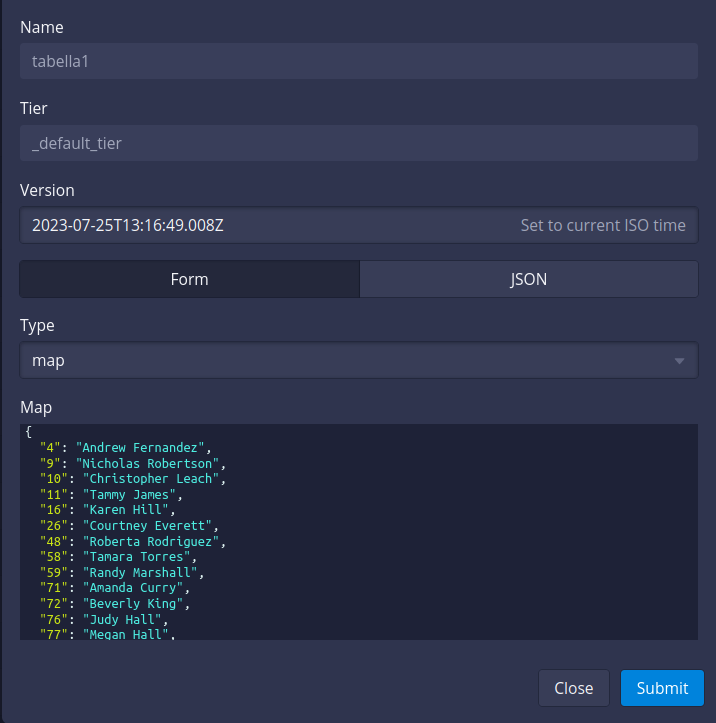
\includegraphics[width=0.6\textwidth]{images/percorso/inserimento_lookup.png}
  \caption{Creazione della tabella di lookup all'interno di Apache Druid}
  \label{fig:lookup}
\end{figure}
\pagebreak
\\
In seguito per poter testare tale funzionalità è stata eseguita la seguente query.
\begin{lstlisting}[language=SQL]
  SELECT LOOKUP(codice_cliente,'tabella1'), datan, citta, stato
  FROM accessi_lookup
\end{lstlisting}
Si sottolinea che, per poter utilizzare le tabelle di \textbf{lookup} in \textbf{Apache Druid}, 
è necessario
inserire all'interno della query desiderata la funzione \textbf{LOOKUP}, riportando come primo parametro il campo chiave della tabella di \textbf{lookup} e come secondo parametro il nome della tabella stessa.\\
\subsubsection{Risultati}
Il risultato ottenuto è illustrato in Figura \ref{fig:risultato_lookup}.
\begin{figure}[H]
  \centering
  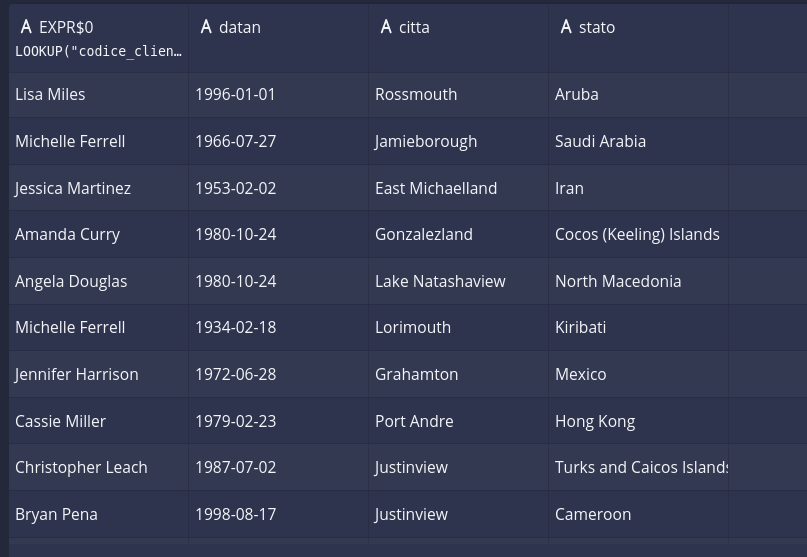
\includegraphics[width=1\textwidth]{images/percorso/lookup.png}
  \caption{Risultato della query eseguita con la funzionalità di lookup}
  \label{fig:risultato_lookup}
\end{figure}
\subsubsection{Considerazioni}
Dai risultati ottenuti 
si sottolinea che per ottenere lo stesso risultato all'interno di un classico \textbf{database relazionale}
è necessario ricorrere all'unione tra due tabelle, operazione che risulta essere molto onerosa.
\newpage
\pagestyle{empty}
\null % o \mbox{} o \phantom{X}
\newpage